\documentclass[hidelinks,12pt,a4paper]{report}
\usepackage[utf8]{inputenc}
\usepackage{amsmath}
\usepackage{amsfonts}
\usepackage{amssymb}
\usepackage[margin=1in,left=1.2in,includefoot]{geometry}
% Algorithm
\usepackage{algorithm}
\usepackage{amssymb}
% IF else
\usepackage{algorithmic}
\usepackage[export]{adjustbox}
\usepackage{caption}


% Hyperlinks
\usepackage{hyperref}
% Graphic
\usepackage{graphicx}
\usepackage{subfig}
\usepackage{float}
\renewcommand{\arraystretch}{2.5}
%----------------------------------------------------------------------------------------
%	DOCUMENT INFORMATION
%----------------------------------------------------------------------------------------

\title{}
\author{Tu \textsc{Vu}}
\date{\today}

\begin{document}

\begin{titlepage}

\includegraphics[height=1.75cm, valign=c]{images/bordeaux_logo.jpg}
\hspace*{0.3cm}
\includegraphics[height=1.75cm, valign=c]{images/LaBRI_logo.jpg}
\hspace*{1.3cm}
\includegraphics[height=1.95cm, valign=c]{images/puf_logo.jpg}\\[1.5cm]
		
	\begin{center}
	
	%\textsc{\LARGE }\\[1.5cm] % Main heading such as the name of your university/college
	
	\textsc{\Large UNIVERSITY OF BORDEAUX}\\[1.5cm] % Major heading such as course name
	
	\textsc{\large INTERNSHIP REPORT}\\[1.5cm] % Minor heading such as course title


%{\large Final report}\\[0.5cm]	
	
	\line(1,0){400}\\[0.2in]
	\huge{\bfseries Deep Learning}\\
	\line(1,0){400}\\[1.5cm]
	\noindent	
	\begin{minipage}{0.4\textwidth}
		\begin{flushleft} \large
    	\emph{Student:}\\
    	Manh Tu \textsc{Vu}
		\end{flushleft}
	\end{minipage}
	\begin{minipage}{0.4\textwidth}
  		\begin{flushright} \large
    		\emph{Supervisor:} \\
    		Marie \textsc{Beurton-Aimar}
    		Van Linh \textsc{Le}
  		\end{flushright}
	\end{minipage}
	
	\vfill

% Bottom of the page
{\large \today}
	\end{center}
\end{titlepage}

% Table content
\tableofcontents
\thispagestyle{empty}
\clearpage
\chapter{Introduction}
Heritage Observatory project has for aim to identify cultural and historical heritages, constitute a specific database, provide a data archive free for all. This platform allows us to receive the breaking news about cultural or historical heritage sites located in regions of the world that we are interesting. In order to do that, the platform will collect a huge of images about the cultural and historical heritage. The problem appears when we want to categorize those images into a specific classes when the image have no label and we can't looking to each of those images and categorize it by hand. We need to find a way to let the computer do it for us.
The aim of my internship is to implement a deep-learning algorithm to classify those images.
\\
\\
Image classification is the task of assigning an input image one label from a fixed set of categories. There are lots of classifiers that exists, but nowadays, neural networks and deep learning currently provide the best solutions to many problems in image and speech recognition, and in natural language processing.
\\
\\
Deep learning, is a part of machine learning and it gives techniques for learning in neural networks. Neural networks are inspired by the human system of neurons that is able to learn from observations. It is feed by labeled data and learns automatically from that. The most adapted neural network for image recognition is the convolutional neural network (CNN). It's adapted to the recognition of 4 classes: being, heritage, scenery and other. That's why it has been implanted.
\\
\\
Deep learning has two major categories of image classification techniques include unsupervised and supervised classification. With unsupervised classification, all images are unlabeled and we using deep learning to learn to inherent structure from the image input data while with supervised classification, all images are labeled and we using deep learning to learn to predict the output from the image input data.
\\
In this project, we'll implement both of those categories of image classification techniques and then compare the result to see which one are better to solve our problem.
\chapter{Context}
\section{Pôle Universitaire Français}
The Pôle Universitaire Français (PUF) was created by the intergovernmental agreement of VietNam and France in October 2004. With ambition is building a linking program between the universities in VietNam and the advanced programs of universities in France. There are two PUF’s center in VietNam: Pôle Universitaire Français de l’Universite Nationalé du Vietnam - Ha Noi located in Ha Noi capital (PUF-Ha Noi) and Pôle Universitaire Français de l’Universite Nationalé du Vietnam - Ho Chi Minh Ville located in Ho Chi Minh city (PUF-HCM).
\subsection{PUF-HCM}
PUF-HCM 1 is a department of VietNam National Univeristy at Ho Chi Minh city. From the first year of operations, PUF-HCM launched the quality training programs from France in VietNam. With target, bring the programs which designed and evaluated by the international standards for Vietnamese student. PUF-HCM always strive in our training work. So far, PUF-HCM have five linking programs with the universities in France, and the programs are organized into the subjects: Commerce, Economic, Management and Informatics. In detail:

\begin{itemize}
	\item Bachelor and Master of Economics : linking program with University of Toulouse 1 Captiole
	\item Bachelor and Master of Informatics: linking program with University of Bordeaux and University of Paris 6.
\end{itemize}
The courses in PUF-HCM are provided in French, English and Vietnamese by both Vietnamese and French professors. The highlight of the programs are inspection and diploma was done by the French universities.
\section{Laboratoire Bordelais de Recherche en Informatique}
The Laboratoire Bordelais de Recherche en Informatique (LaBRI) 2 is a research unit associated with the CNRS (URM 5800), the University of Bordeaux and the Bordeaux INP. Since 2002, it has been the partner of Inria. It has significantly increased in staff numbers over recent years.
In March 2015, it had a total of 320 members including 113 teaching/research staff (University of Bordeaux and Bordeaux INP), 37 research staff (CNRS and Inria), 22 administrative and technical (University of Bordeaux, Bordeaux INP, CNRS and Inria) and more than 140 doctoral
students and post-docs. The LaBRI’s missions are: research (pure and applied), technology application and transfer and training.
Today the members of the laboratory are grouped in six teams, each one combining basic research, applied research and technology transfer:
\begin{itemize}
	\item Combinatorics and Algorithmic
	\item Image and Sound
	\item Formal Methods
	\item Models and Algorithms for Bio-informatics and Data Visualisation
	\item Programming, Networks and Systems
	\item Supports and Algorithms for High Performance Numerical Applications
\end{itemize}
Within these team, research activities are conducted in partnership with Inria. Besides that, LaBRI also collaborate with many other laboratories and companies on French, European and the international.

\chapter{Aglorithm to solve our problem}
In this part, we will explain how we choose the aglorithms to solve our problem and describe what is each one.
\section{Scikit-learn algorithm cheat-sheet\cite{scikitlearn.org}}
Because it has many algorithms has able to classify images such as: Decision tree\cite{j.r.quinlan1985}, SVM\cite{stever.gunn1998}, K-nearest neighbors\cite{orenanavakfiry.levy2017}, etc. We need to find a right one to solve our problem. The Scikit-learn had made an algorithm cheat-sheet to help us to choose the right one:

\begin{figure}[ht]
	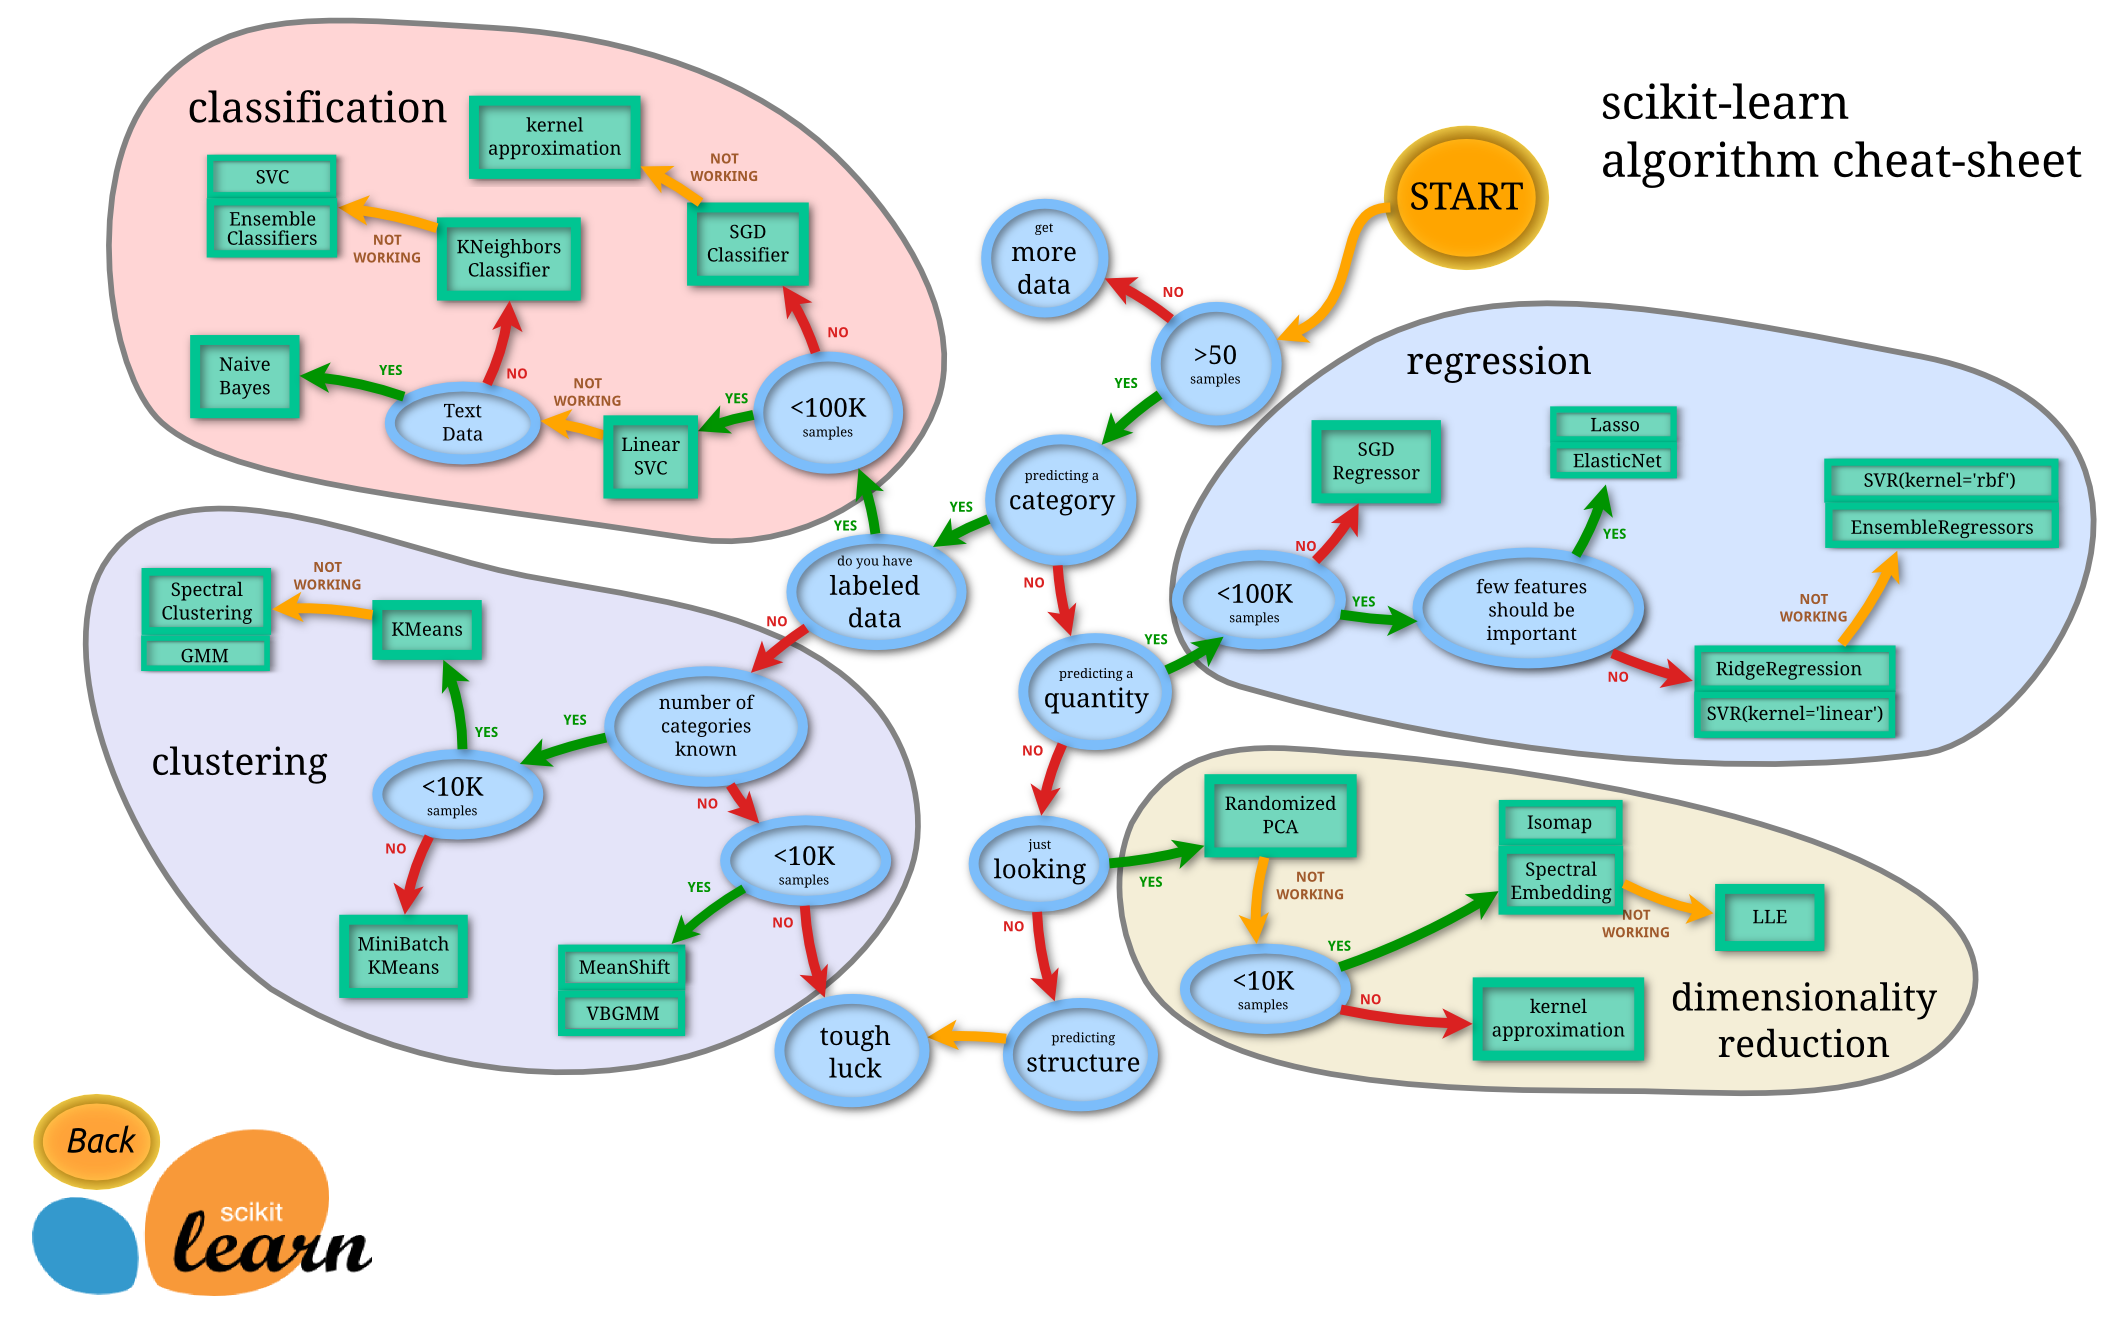
\includegraphics[width=\textwidth, center]{images/scikit-learn}
	\caption{Scikit-learn algorithm cheat-sheet}
	\label{fig:Scikit-learn}
\end{figure}
As the Fig \ref{fig:Scikit-learn} above, we'll use K-mean algorithm to classify our images. However, we can create a labeled dataset from our unlabeled images by hand. So, we can also use SGD Classifier to solve our problem.
\\
Finally, this lead us to two ways: one is use Supervised Classification with SGD is our main algorithm. The second is use Unsupervised Classification with K-mean is main algorithm.
\section{General architecture}
A convolutional network is a neural network that use convolutions. It is a multiplayer network (e. g. it uses several layers). In reality, those kind of network, are dividing in two part. The first one use convolutional layers - layers that use convolution patches to compute weights used in neurons. The second part, used to connect the first part to the output, is made of fully connected layers: every output of a layer is connected to every neurons of the next one without any distinctions.

\begin{figure}[ht]
	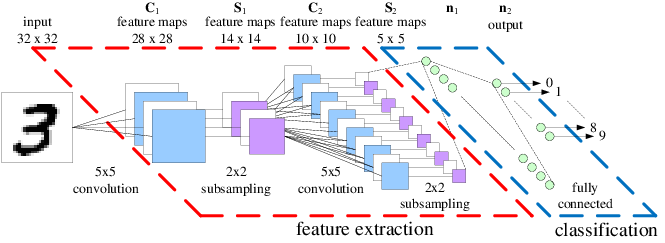
\includegraphics[scale=1, center]{images/Fig-1-An-Example-CNN-architecture-for-a-handwritten-digit-recognition-task}
	\caption{An Example CNN architecture for a handwritten digit recognition task.}
	\label{fig:CNN-architecture}
\end{figure}
The network architecture of an example CNN is depicted in Fig \ref{fig:CNN-architecture}. The processing starts with feature extraction layers and is finished by fully connected classification layers. Using different layers delivers robust recognition accuracy and is invariant to small geometric transformations of the input images. The robust recognition accuracy makes that CNN are successfully used for classification tasks on real world data

\chapter{The internship project: Research in Deep Learning}

The internship is intended to be a duration to apply the knowledge to the real environment. It shows the ability synthesis, evaluation and self-research of student. Besides, the student may study the experience from the real working environment. My internship is done under the
guidance of Mrs Marie BEURTON-AIMAR in a period of six months at LaBRI laboratory.
The project is working on the Image Classification field. The goal of the project is using Deep Learning to classify all images from \href{https://heobs.org}{https://heobs.org} into 4 classes, include:
\begin{description}
\item[Heritage] \hfill \\ A place of cultural, historical, or natural significance for a group or society.
\item[Beings] \hfill \\ Any form of life, such as a plant or a living creature, whether human or other animal.
\item[Scenery] \hfill \\ Any form of landscapes which show little or no human activity and are created in the pursuit of a pure, unsullied depiction of nature, also known as scenery.
\item[Other] \hfill \\ Any other type of image that doesn't represent a photograph, such as painting, illustration, any object.	
\end{description}
The administrator of \href{https://heobs.org}{https://heobs.org} has collected a set of 144564 images about vietnamese human, statue, ancient artifacts, building, landscape, etc. But all of them are completed unlabeled. So, the question is: ``How we can classify those images to the right classes and how to automatic classify the new image, which the machine has never seen to the right class''.\\
The objective of this internship is implementing a method to automatic classify images.
The method is use deep convolutional neural networks (CNNs or ConvNets) to tackle the remote sensing scene classification task.

\begin{figure}[!htb]
\minipage{0.32\textwidth}
  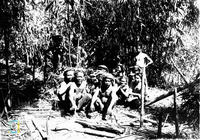
\includegraphics[height=3.5cm, left]{images/sample/being_6}
  \captionsetup{labelformat=empty}
  \caption{Being}
\endminipage\hfill
\minipage{0.32\textwidth}
  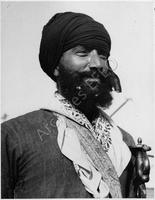
\includegraphics[height=3.5cm, center]{images/sample/being_35}
  \captionsetup{labelformat=empty}
  \caption{Being}
\endminipage\hfill
\minipage{0.32\textwidth}%
  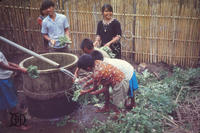
\includegraphics[height=3.5cm, right]{images/sample/being_45}
  \captionsetup{labelformat=empty}
  \caption{Being}
\endminipage
\end{figure}

\begin{figure}[!htb]
\minipage{0.32\textwidth}
  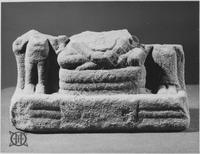
\includegraphics[width=5.2cm, height=3.5cm, left]{images/sample/heritage_145}
  \captionsetup{labelformat=empty}
  \caption{Heritage}
\endminipage\hfill
\minipage{0.32\textwidth}
  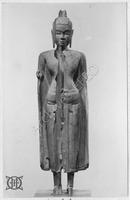
\includegraphics[height=3.5cm, center]{images/sample/heritage_147}
  \captionsetup{labelformat=empty}
  \caption{Heritage}
\endminipage\hfill
\minipage{0.32\textwidth}%
  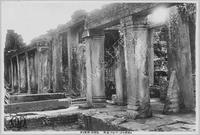
\includegraphics[width=5.2cm, height=3.5cm, right]{images/sample/heritage_282}
  \captionsetup{labelformat=empty}
  \caption{Heritage}
\endminipage
\end{figure}

\begin{figure}[!htb]
\minipage{0.32\textwidth}
  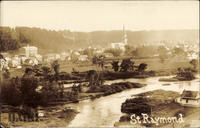
\includegraphics[height=2.8cm, left]{images/sample/scenery_111}
  \captionsetup{labelformat=empty}
  \caption{Scenery}
\endminipage\hfill
\minipage{0.32\textwidth}
  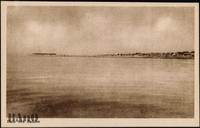
\includegraphics[height=2.8cm, center]{images/sample/scenery_102}
  \captionsetup{labelformat=empty}
  \caption{Scenery}
\endminipage\hfill
\minipage{0.32\textwidth}%
  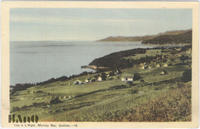
\includegraphics[height=2.8cm, right]{images/sample/scenery_110}
\captionsetup{labelformat=empty}
  \caption{Scenery}
\endminipage
\end{figure}

\begin{figure}[!htb]
\minipage{0.32\textwidth}
  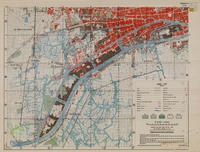
\includegraphics[width=5.2cm, height=3.5cm, left]{images/sample/other_129}
  \captionsetup{labelformat=empty}
  \caption{Other}
\endminipage\hfill
\minipage{0.32\textwidth}
  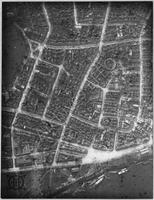
\includegraphics[height=3.5cm, center]{images/sample/other_190}
  \captionsetup{labelformat=empty}
  \caption{Other}
\endminipage\hfill
\minipage{0.32\textwidth}%
  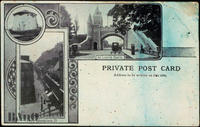
\includegraphics[width=5.2cm, height=3.5cm, right]{images/sample/other_202}
  \captionsetup{labelformat=empty}
  \caption{Other}
\endminipage
  \caption{Images from heobs.org}
\end{figure}

\bibliographystyle{ieeetr}
\bibliography{bibfile}
\end{document}